%% abtex2-modelo-relatorio-tecnico.tex, v-1.7.1 laurocesar
%% Copyright 2012-2013 by abnTeX2 group at http://abntex2.googlecode.com/ 
%%
%% This work may be distributed and/or modified under the
%% conditions of the LaTeX Project Public License, either version 1.3
%% of this license or (at your option) any later version.
%% The latest version of this license is in
%%   http://www.latex-project.org/lppl.txt
%% and version 1.3 or later is part of all distributions of LaTeX
%% version 2005/12/01 or later.
%%
%% This work has the LPPL maintenance status `maintained'.
%% 
%% The Current Maintainer of this work is the abnTeX2 team, led
%% by Lauro César Araujo. Further information are available on 
%% http://abntex2.googlecode.com/
%%
%% This work consists of the files abntex2-modelo-relatorio-tecnico.tex,
%% abntex2-modelo-include-comandos and abntex2-modelo-references.bib
%%

% ------------------------------------------------------------------------
% ------------------------------------------------------------------------
% abnTeX2: Modelo de Relatório Técnico/Acadêmico em conformidade com 
% ABNT NBR 10719:2011 Informação e documentação - Relatório técnico e/ou
% científico - Apresentação
% ------------------------------------------------------------------------ 
% ------------------------------------------------------------------------

% Alterado por Rodrigo Campiolo para apresentação de relatórios na disciplina
% de Redes de Computadores II do Bacharelado em Ciência da Computação da UTFPR-CM.


\documentclass[
	% -- opções da classe memoir --
	12pt,				% tamanho da fonte
	%openright,			% capítulos começam em pág ímpar (insere página vazia caso preciso)
	oneside,   	        % para impressão em verso e anverso use twoside. Oposto a oneside
	a4paper,			% tamanho do papel. 
	% -- opções da classe abntex2 --
	%chapter=TITLE,		% títulos de capítulos convertidos em letras maiúsculas
	%section=TITLE,		% títulos de seções convertidos em letras maiúsculas
	%subsection=TITLE,	% títulos de subseções convertidos em letras maiúsculas
	%subsubsection=TITLE,% títulos de subsubseções convertidos em letras maiúsculas
	% -- opções do pacote babel --
	english,			% idioma adicional para hifenização
	french,				% idioma adicional para hifenização
	spanish,			% idioma adicional para hifenização
	brazil,				% o último idioma é o principal do documento
	]{pacotes/abntex2}


% ---
% PACOTES
% ---

% ---
% Pacotes fundamentais 
% ---
\usepackage{cmap}				% Mapear caracteres especiais no PDF
\usepackage{lmodern}			% Usa a fonte Latin Modern
\usepackage[T1]{fontenc}		% Selecao de codigos de fonte.
\usepackage[utf8]{inputenc}		% Codificacao do documento (conversão automática dos acentos)
\usepackage{indentfirst}		% Indenta o primeiro parágrafo de cada seção.
\usepackage{color}				% Controle das cores
\usepackage{graphicx}			% Inclusão de gráficos
% ---

% ---
% Pacotes adicionais, usados no anexo do modelo de folha de identificação
% ---
\usepackage{multicol}
\usepackage{multirow}
% ---
	
% ---
% Pacotes adicionais, usados apenas no âmbito do Modelo Canônico do abnteX2
% ---
\usepackage{lipsum}				% para geração de dummy text
% ---

% ---
% Pacotes de citações
% ---
\usepackage[brazilian,hyperpageref]{backref}	 % Paginas com as citações na bibl
\usepackage[alf]{pacotes/abntex2cite}	% Citações padrão ABNT
\usepackage{comment}
% ---

% ---
% Meus pacotes
% ---
\usepackage{float}
% ---

% --- 
% CONFIGURAÇÕES DE PACOTES
% --- 

% ---
% Configurações do pacote backref
% Usado sem a opção hyperpageref de backref
\renewcommand{\backrefpagesname}{Citado na(s) página(s):~}
% Texto padrão antes do número das páginas
\renewcommand{\backref}{}
% Define os textos da citação
\renewcommand*{\backrefalt}[4]{
	\ifcase #1 %
		Nenhuma citação no texto.%
	\or
		Citado na página #2.%
	\else
		Citado #1 vezes nas páginas #2.%
	\fi}%
% ---

% ---
% Informações de dados para CAPA e FOLHA DE ROSTO
% ---
\titulo{Instalar o GNU/Linux e compilar o núcleo}
\autor{Hendrick Felipe Scheifer\\João Victor Briganti\\Luiz Gustavo Takeda}
\local{Campo Mourão}
\data{Outubro / 2024}
\instituicao{%
  Universidade Tecnológica Federal do Paraná -- UTFPR
  \par
  Departa           mento Acadêmico de Computação -- DACOM
  \par
  Bacharelado em Ciência da Computação -- BCC
}
\tipotrabalho{Relatório técnico}
% O preambulo deve conter o tipo do trabalho, o objetivo, 
% o nome da instituição e a área de concentração 
\preambulo{Relatório técnico de atividade prática solicitado pelo professor Rodrigo Campiolo na disciplina de Sistemas Operacionais do Bacharelado em Ciência da Computação da Universidade Tecnológica Federal do Paraná.}
% ---

% ---
% Configurações de aparência do PDF final

% alterando o aspecto da cor azul
\definecolor{blue}{RGB}{41,5,195}

% informações do PDF
\makeatletter
\hypersetup{
     	%pagebackref=true,
		pdftitle={\@title}, 
		pdfauthor={\@author},
    	pdfsubject={\imprimirpreambulo},
	    pdfcreator={LaTeX with abnTeX2},
		pdfkeywords={abnt}{latex}{abntex}{abntex2}{relatório técnico}, 
		colorlinks=true,       		% false: boxed links; true: colored links
    	linkcolor=blue,          	% color of internal links
    	citecolor=blue,        		% color of links to bibliography
    	filecolor=magenta,      		% color of file links
		urlcolor=blue,
		bookmarksdepth=4
}
\makeatother
% --- 

% --- 
% Espaçamentos entre linhas e parágrafos 
% --- 

% O tamanho do parágrafo é dado por:
\setlength{\parindent}{1.3cm}

% Controle do espaçamento entre um parágrafo e outro:
\setlength{\parskip}{0.2cm}  % tente também \onelineskip

% ---
% compila o indice
% ---
\makeindex
% ---

% Omite a numeração de capítulos
\renewcommand*\thesection{\arabic{section}}



% ----
% Início do documento
% ----
\begin{document}

% Retira espaço extra obsoleto entre as frases.
\frenchspacing 

% ----------------------------------------------------------
% ELEMENTOS PRÉ-TEXTUAIS
% ----------------------------------------------------------
% \pretextual

% ---
% Capa
% ---
%\imprimircapa
% ---

% ---
% Folha de rosto
% (o * indica que haverá a ficha bibliográfica)
% ---
\imprimirfolhaderosto
% ---


% ---
% RESUMO
% ---

% resumo na língua vernácula (obrigatório)
\begin{resumo}
Este trabalho apresenta os procedimentos necessários para a instalação de uma distribuição GNU/Linux, focando na configuração e compilação do núcleo do sistema operacional. Utilizou-se o hipervisor VirtualBox (versão 7.1.2) para criar uma máquina virtual, na qual foi instalada a distribuição Debian (versão $12.7$) e o núcleo Linux (versão $6.10.11$). Durante o processo, foram executados diversos comandos básicos, possibilitando uma compreensão aprofundada da estrutura do sistema e a aplicação prática dos conceitos aprendidos em sala de aula. Os resultados evidenciam a importância da prática na consolidação do conhecimento teórico.

 \vspace{\onelineskip}
    
 \noindent
 \textbf{Palavras-chave}: VirtualBox. Debian. Sistema Operacional.
\end{resumo}
% ---

% ---
% inserir lista de ilustrações
% ---
%\pdfbookmark[0]{\listfigurename}{lof}
%\listoffigures*
%\cleardoublepage
% ---

% ---
% inserir lista de tabelas
% ---
%\pdfbookmark[0]{\listtablename}{lot}
%\listoftables*
%\cleardoublepage
% ---

% ---
% inserir lista de abreviaturas e siglas
% ---
%\begin{siglas}
%  \item[IP] Internet Protocol
%  \item[TCP] Transmission Control Protocol
%  \item[UDP] User Datagram Protocol
%\end{siglas}
% ---

% ---
% inserir o sumario
% ---
\pdfbookmark[0]{\contentsname}{toc}
\tableofcontents*
\cleardoublepage
% ---

% ----------------------------------------------------------
% ELEMENTOS TEXTUAIS
% ----------------------------------------------------------
\textual

\makeatletter
\renewcommand{\chapter}{\@gobbletwo}
\makeatother

\section{Introdução}
\label{sec:introducao}
Um sistema operacional é um dispositivo de \textit{software} cuja função é tornar o computador mais simples e limpo, além de ser responsável pelo gerenciamento dos recursos da máquina~\cite{tanenbaum2016}.

A maioria dos computadores possui dois modos de operação: modo núcleo e modo usuário. O sistema operacional é um \textit{software} que opera em modo núcleo, garantindo acesso total ao \textit{hardware}, possibilitando a execução de qualquer instrução suportada pela máquina utilizada~\cite{tanenbaum2016}.

Este trabalho está estruturado da seguinte forma: após a introdução serão apresentados os objetivos do trabalho; em seguida, uma breve fundamentação essencial para o pleno entendimento do trabalho será apresentada; após isso, serão apresentados os materiais utilizados para a realização do trabalho, na seção 4; na seção 5, serão apresentadas e explicadas as etapas realizadas durante esta atividade; a seguir, na seção 6 e 7, os resultados serão discutidos e será apresentado as conclusões do trabalho, respectivamente.

\section{Objetivos}
\label{sec:objetivos}

Este trabalho visa instalar a distribuição GNU/Linux Debian em um ambiente virtual, compilar e instalar o núcleo Linux, e explicar detalhadamente cada um dos comandos utilizados durante todo o procedimento.

\section{Fundamentação}
\label{sec:fundamentacao}

A primeira versão do Linux foi desenvolvida por Linus Torvalds em 1991, como um sistema operacional para computadores que utilizavam o microprocessador, Intel 80386, que era um processador novo e o mais avançado da época. A parte mais interna de um sistema operacional é denominada núcleo, um \textit{software} que fornece serviços básicos para todas as outras partes do sistema, gerencia o \textit{hardware} e distribui recursos do sistema~\cite{robert2010}.

Como o código-fonte do Linux é aberto, podemos configurá-lo antes de compilarmos, escolhendo apenas os \textit{drivers} e conteúdos específicos que desejamos~\cite{robert2010}. Uma distribuição GNU/Linux possui uma combinação específica de \textit{softwares} aliados ao núcleo, o qual pode ser customizado conforme a necessidade. A distribuição utilizada para esta atividade é denominada GNU/Linux Debian.

\section{Materiais}
\label{sec:materiais}

\begin{itemize}
  \item Especificações do computador utilizado:
  \begin{itemize}
    \item Modelo: Notebook Lenovo Thinkpad E14
    \item CPU: AMD Ryzen $5$-$3500$U
    \item Memória Principal: $8$GB RAM
    \item Memória Secundária: SSD $256$ NVME
    \item Sistema Operacional: Fedora $40$
  \end{itemize}
  \item Hipervisor: VirtualBox $7.1.2$
  \item Sistema Operacional utilizado no Hipervisor: GNU/Linux Debian $12.7$
  \item Núcleo: Linux $6.10.11$
\end{itemize}

\section{Procedimentos e Resultados}
\label{sec:procedimentos}

Nesta seção, serão detalhados os procedimentos executados para a instalação da distribuição GNU/Linux Debian em um ambiente virtual, utilizando o hipervisor VirtualBox. Serão abordadas as configurações iniciais do hipervisor, a instalação do sistema operacional, verificações essenciais e os comandos utilizados para garantir o funcionamento correto do ambiente. Além disso, será descrito o processo de compilação do núcleo Linux, incluindo as etapas necessárias para a personalização e instalação da nova versão. 

\subsection{Configurações do Hipervisor}
\label{subsec:hipervisor}

Os passos iniciais se deram por meio da instalação do Oracle VM VirtualBox e também da obtenção da imagem do Debian que foi utilizada para a instalação. 

\begin{figure}[H]
  \centering
  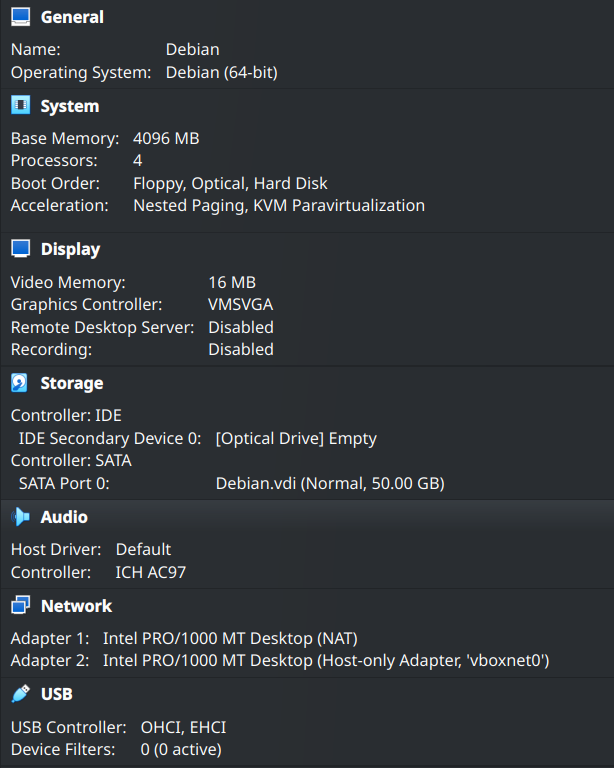
\includegraphics[scale=0.7]{figuras/vm.png}
  \caption{Configurações do hipervisor.}
  \label{fig:vm}
\end{figure}

A Figura~\ref{fig:vm} ilustra as principais configurações utilizadas para a instalação do sistema operacional. Para a memória primária, foi selecionado um total de 4 GB e 4 processadores, enquanto a memória secundária foi alocada com 50 GB para uso da máquina virtual.

Além das configurações de processadores e memória, foram incluídas duas placas de rede. O adaptador 1 está configurado como Network Address Translation (NAT), permitindo acesso à Internet, enquanto o adaptador 2 está configurado para uso interno. Essa configuração foi escolhida pois o acesso à máquina será realizado por meio do Secure Shell Connection (SSH).

\subsection{Instalação do Sistema Operacional}
\label{subsec:instalacao}

Os primeiros passos durante a instalação envolveram a seleção do idioma. Para facilitar a referência a manuais durante o processo, optou-se pelo inglês. Após essa configuração, o Brasil foi escolhido como localização, permitindo que o sistema operacional definisse o \textit{locale} a ser utilizado para formatações específicas relacionadas à região do usuário~\cite{kerris2010}. Além disso, o relógio do sistema foi ajustado para o fuso horário de São Paulo, e o teclado foi configurado para a disposição adequada da região.

Após as configurações de região, foram criados um usuário comum e um usuário \textit{root}. Na Figura~\ref{fig:root} temos a descrição do \textit{root}, administrador do sistema, possuindo privilégios amplos e acesso total a todos os recursos e configurações do sistema.

\begin{figure}[H]
  \centering
  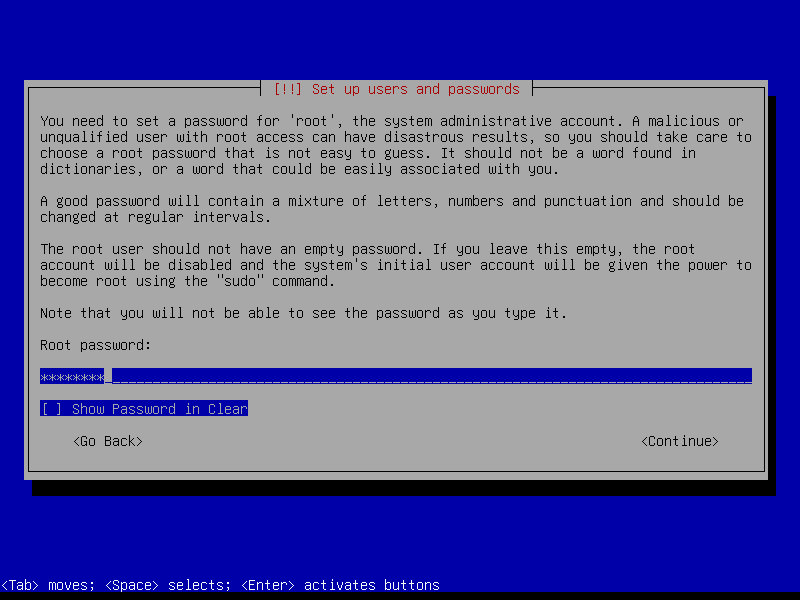
\includegraphics[scale=0.7]{figuras/root.png}
  \caption{Criação do usuário \textit{root}.}
  \label{fig:root}
\end{figure}

Na Figura~\ref{fig:partition}, estão apresentadas as configurações de particionamento e pontos de montagem do disco. O particionamento permite a divisão entre partições primárias e lógicas, sendo que cada uma delas é derivada do Master Boot Record (MBR). De maneira simplificada, as partições primárias são inicializáveis, enquanto as partições lógicas existem apenas como uma forma de contornar algumas limitações existentes na divisão das partições~\cite{negus2012}.

A memória secundária possui 50 GB de armazenamento, o que possibilitou que as partições fossem dispostas da seguinte maneira:

\begin{itemize}
    \item \textit{/}: É a raiz do sistema de arquivos, servindo como ponto de montagem para todos os outros dispositivos e sistemas de arquivos. Por ser o local onde o sistema operacional inicia e onde estão armazenados arquivos críticos, foi alocado um tamanho de 4 GB para esta partição.
    
    \item \textit{/usr}: Este diretório é responsável por armazenar programas e dados de usuários. Por conter a maior quantidade de dados e ser amplamente utilizado durante a compilação, foi escolhido um tamanho de 5 GB para esta partição.
    
    \item \textit{/var}: Armazena dados variáveis, como logs e outros arquivos que podem mudar com frequência. Por não ser uma área crítica para o funcionamento do sistema, neste trabalho em específico, foi definido um tamanho de apenas 2 GB.
    
    \item \textit{swap}: Esta partição é utilizada para armazenar páginas de memória que estavam na RAM, funcionando como uma extensão da memória virtual do sistema. Devido à quantidade de RAM já alocada durante a configuração do hipervisor, optou-se por um tamanho de apenas 500 MB para a partição \textit{swap}.
    
    \item \textit{/home}: Este diretório armazena os arquivos de configuração pessoal de cada usuário do sistema. Como é uma área frequentemente utilizada pelos usuários, foi definido um tamanho maior do que o das demais partições, totalizando 10 GB.
\end{itemize}

\begin{figure}[H]
  \centering
  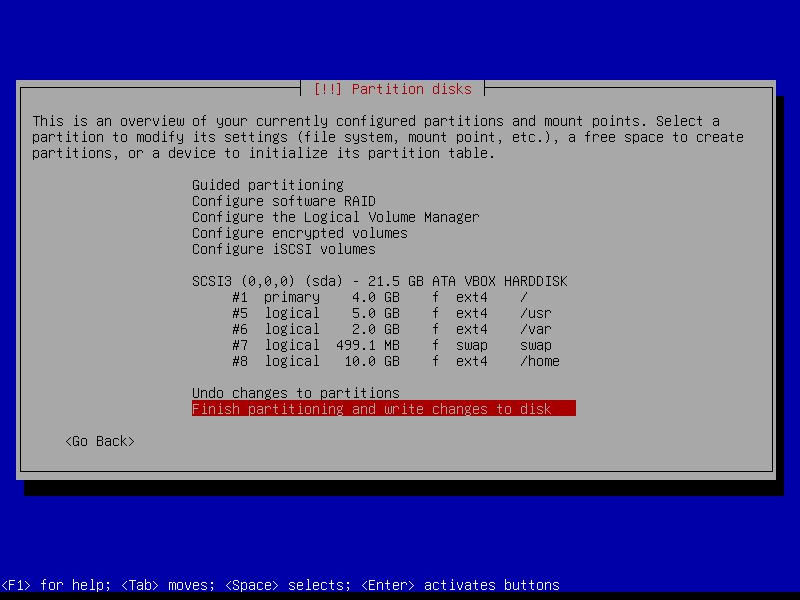
\includegraphics[scale=0.7]{figuras/partition.png}
  \caption{Partições do sistema.}
  \label{fig:partition}
\end{figure}

\subsection{Verificações e Comandos}
\label{subsec:verificacao}

Após o processo de instalação, alguns comandos foram realizados para verificação e teste do sistema instalado.

\subsubsection{ps aux}
A Figura~\ref{fig:ps}, mostra a saída do comando \textit{ps} utilizado para a verificação dos processos em execução no sistema~\cite{negus2012}. A opção ``aux'', é uma divisão de três parâmetros que alteram o comando da seguinte maneira:

\begin{itemize}
    \item 'a': Mostra os processo de todos os usuários.
    
    \item 'u': Altera o formato da saída do programa.
    
    \item 'x': Inclui processos de segundo plano, como \textit{daemons}.
\end{itemize}

\begin{figure}[H]
  \centering
  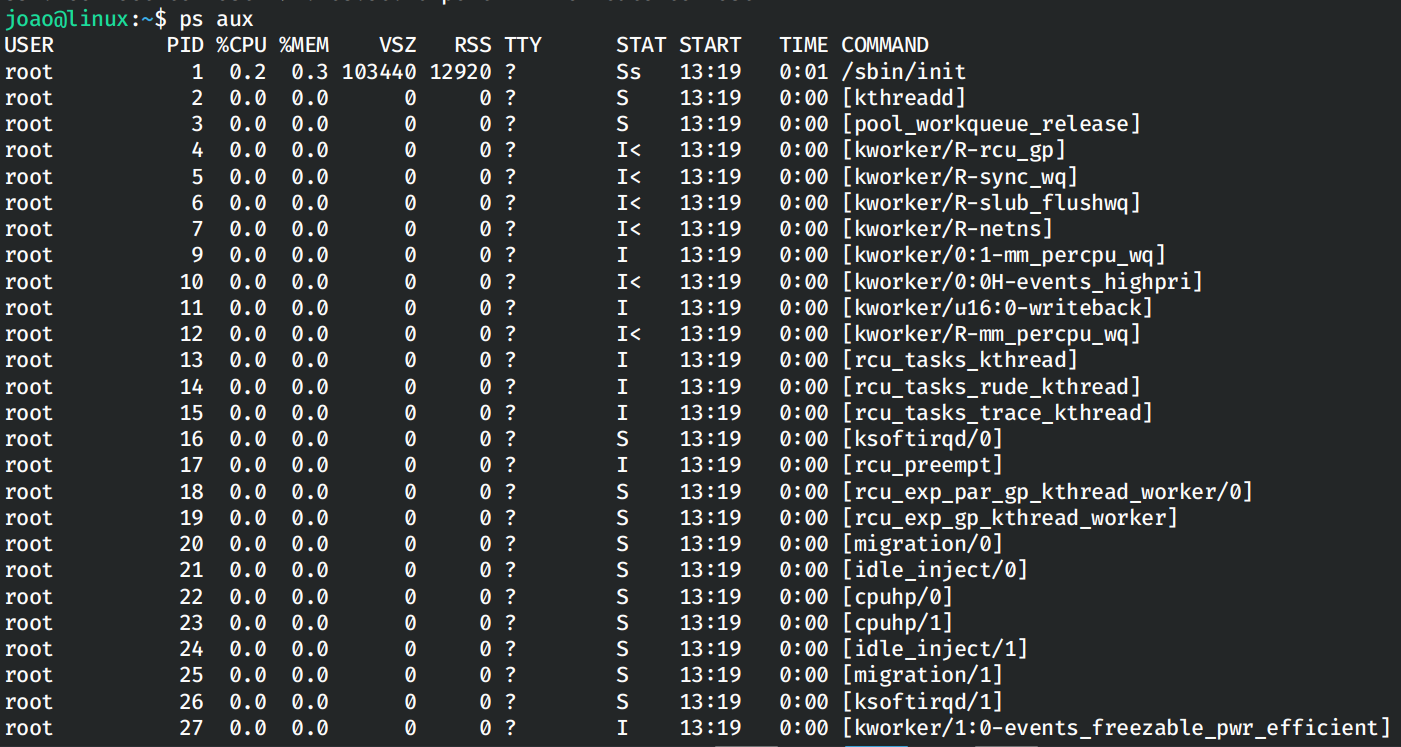
\includegraphics[scale=0.37]{figuras/ps_aux.png}
  \caption{Saída do comando \textit{ps aux}.}
  \label{fig:ps}
\end{figure}

\subsubsection{df}
A Figura~\ref{fig:df} apresenta a saída do comando \textit{df}, utilizado para verificar o espaço utilizado pelos sistemas de arquivos no sistema~\cite{negus2012}. A opção ``-h'' exibe a saída de maneira mais legível, facilitando a interpretação dos dados.

\begin{figure}[H]
  \centering
  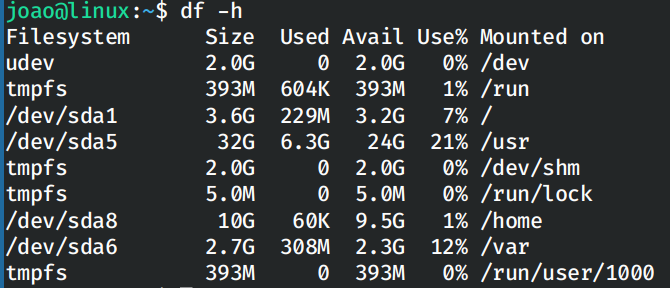
\includegraphics[scale=0.5]{figuras/df.png}
  \caption{Saída do comando \textit{df -h}.}
  \label{fig:df}
\end{figure}

\subsubsection{free}
A Figura~\ref{fig:free} apresenta a saída do comando \textit{free}, utilizado para verificar a utilização da memória no sistema~\cite{shotts2017}. A opção ``-b'' exibe os valores de memória em bytes, proporcionando uma visão detalhada da quantidade exata de memória disponível e utilizada.

\begin{figure}[H]
  \centering
  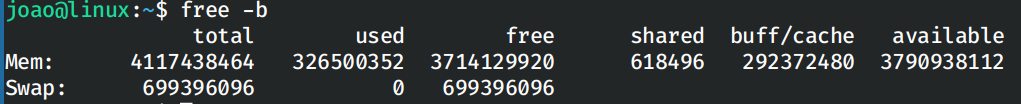
\includegraphics[scale=0.5]{figuras/free.png}
  \caption{Saída do comando \textit{free -b}.}
  \label{fig:free}
\end{figure}

\subsubsection{cat /proc/meminfo}
A Figura~\ref{fig:meminfo} apresenta a saída do comando \textit{cat /proc/meminfo}. O comando \textit{cat} é utilizado para exibir o conteúdo de arquivos de texto no terminal~\cite{shotts2017}. Neste caso, \textit{/proc/meminfo} é um arquivo do sistema que fornece dados em tempo real sobre a utilização da memória física e da \textit{swap}~\cite{tldpProc}.

\begin{figure}[H]
  \centering
  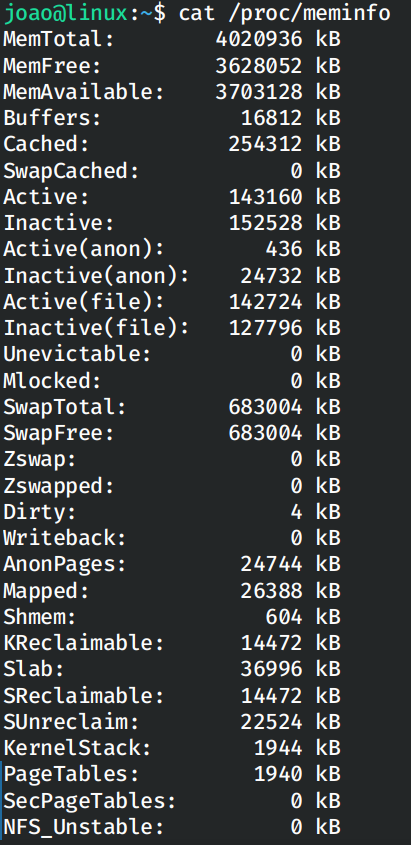
\includegraphics[scale=0.5]{figuras/proc.png}
  \caption{Saída do comando \textit{cat /proc/meminfo}.}
  \label{fig:meminfo}
\end{figure}

\subsubsection{ip}

A Figura~\ref{fig:ip} apresenta as saídas dos comandos \textit{ip -c address show} e \textit{ip -c route}. O comando \textit{ip} é parte das ferramentas do sistema Linux utilizadas para exibir e configurar informações de rede~\cite{manIP}. O parâmetro ''-c`` é utilizado para adicionar cores às saídas, facilitando a leitura das informações.

O comando \textit{ip -c address show} fornece dados importantes, como o endereço Internet Protocol (IP), máscara de rede, \textit{status} das interfaces e outras configurações relevantes.

O comando \textit{ip -c route} exibe a tabela de roteamento.

\begin{figure}[H]
  \centering
  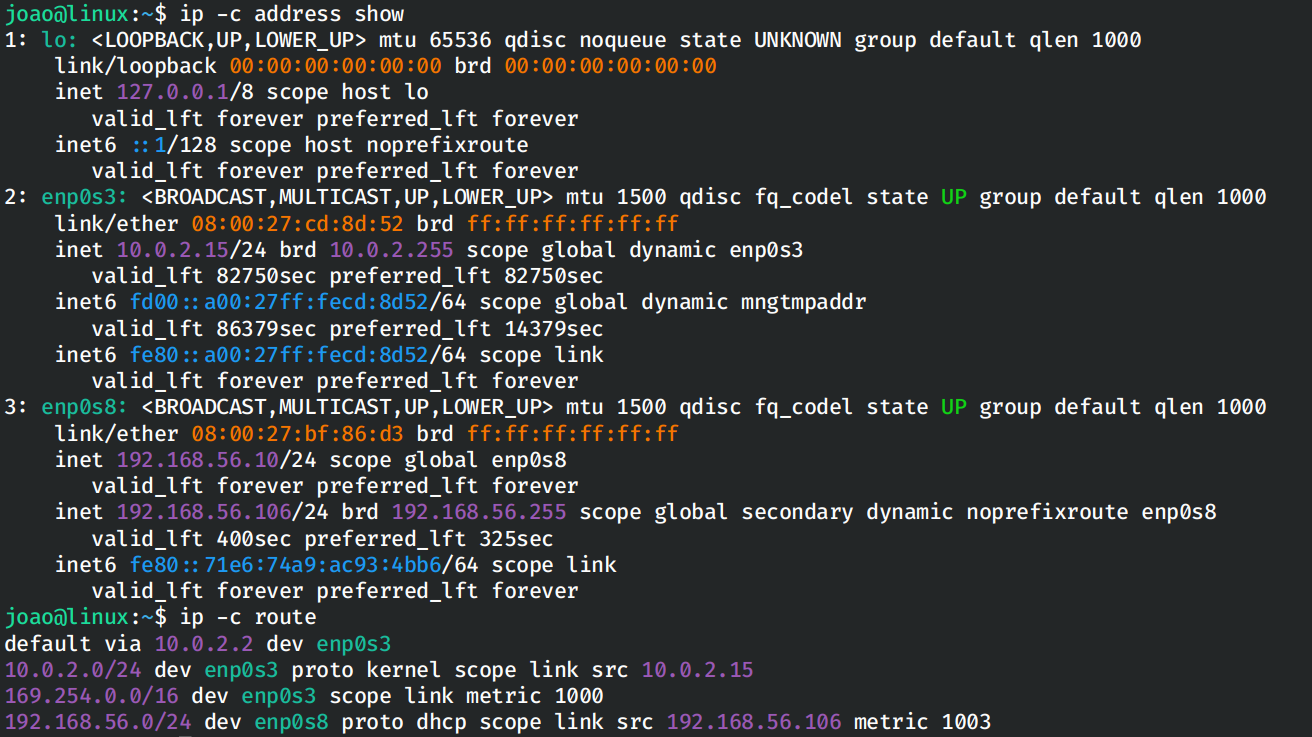
\includegraphics[scale=0.5]{figuras/ip.png}
  \caption{Saídas dos comandos \textit{ip -c address show} e \textit{ip -c route}.}
  \label{fig:ip}
\end{figure}

\subsubsection{cat /etc/resolv.conf}
A Figura~\ref{fig:resolv} mostra a saída do comando \textit{cat /etc/resolv.conf}, que exibe o conteúdo do arquivo responsável pela configuração dos servidores \textit{Domain Name Server} (DNS) no sistema~\cite{negus2012}. Esse arquivo contém informações sobre quais servidores DNS o sistema deve consultar para resolver nomes de domínio em endereços IP.  

\begin{figure}[H]
  \centering
  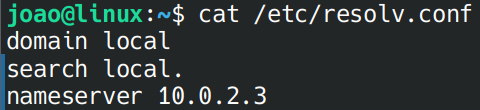
\includegraphics[scale=0.37]{figuras/resolv.png}
  \caption{Conteúdo do arquivo \textit{/etc/resolv.conf}.}
  \label{fig:resolv}
\end{figure}

\subsubsection{cat /etc/network/interfaces}
A Figura~\ref{fig:interfaces} apresenta a saída do comando \textit{cat /etc/network/interfaces}, que exibe as configurações de rede do sistema~\cite{guiafocaIntermediario}. Este arquivo define as interfaces de rede disponíveis e suas configurações, como endereços IP, máscara de sub-rede e gateways.

\begin{figure}[H]
  \centering
  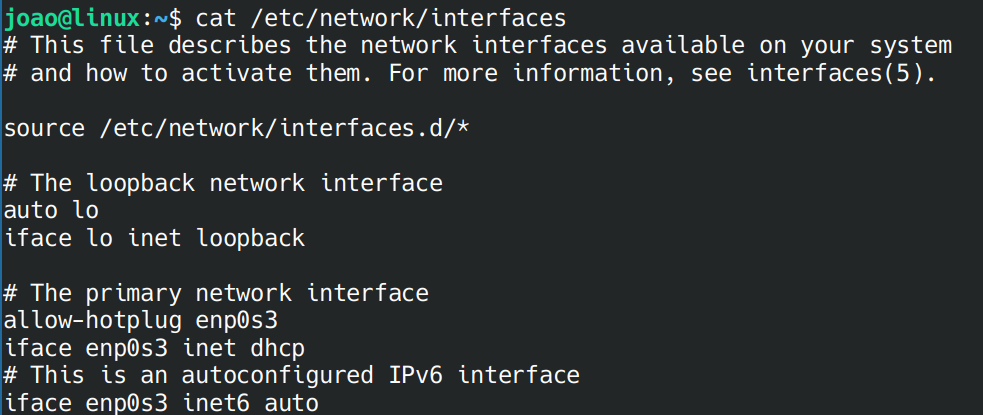
\includegraphics[scale=0.37]{figuras/interfaces.png}
  \caption{Conteúdo do arquivo \textit{/etc/network/interfaces}.}
  \label{fig:interfaces}
\end{figure}

\subsubsection{ping}
A Figura~\ref{fig:ping} mostra a saída do comando \textit{ping google.com}, utilizado para verificar a conectividade com o host especificado~\cite{shotts2017}. O comando envia pacotes ICMP Echo Request para o servidor do Google e mede o tempo de resposta, permitindo avaliar a latência da conexão.

\begin{figure}[H]
  \centering
  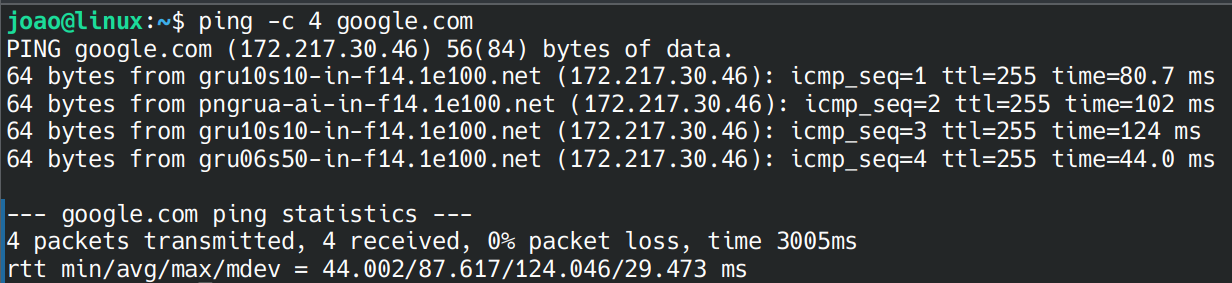
\includegraphics[scale=0.37]{figuras/ping.png}
  \caption{Saída do comando \textit{ping google.com}.}
  \label{fig:ping}
\end{figure}

\subsubsection{Configuração de Repositórios}
O arquivo \textit{sources.list} é um componente essencial do gerenciador de pacotes \textit{apt} no Debian~\cite{guiafocaIniciante}. Neste arquivo é definido os repositórios de onde o sistema obtém os pacotes de software e suas respectivas atualizações. Cada linha do arquivo especifica uma fonte de pacotes, que pode ser um repositório oficial ou um repositório de terceiros.

O \textit{security source list} é uma configuração específica que permite ao sistema acessar repositórios dedicados a atualizações de segurança. Esses repositórios contêm pacotes que corrigem vulnerabilidades e problemas de segurança, sendo fundamental para manter o sistema protegido contra ameaças. 

Como apresentado na Figura~\ref{fig:sources} o Debian 12.7 utilizado neste trabalho, já está previamente configurado com as entradas necessárias para acessar os repositórios principais e de segurança.

\begin{figure}[H]
  \centering
  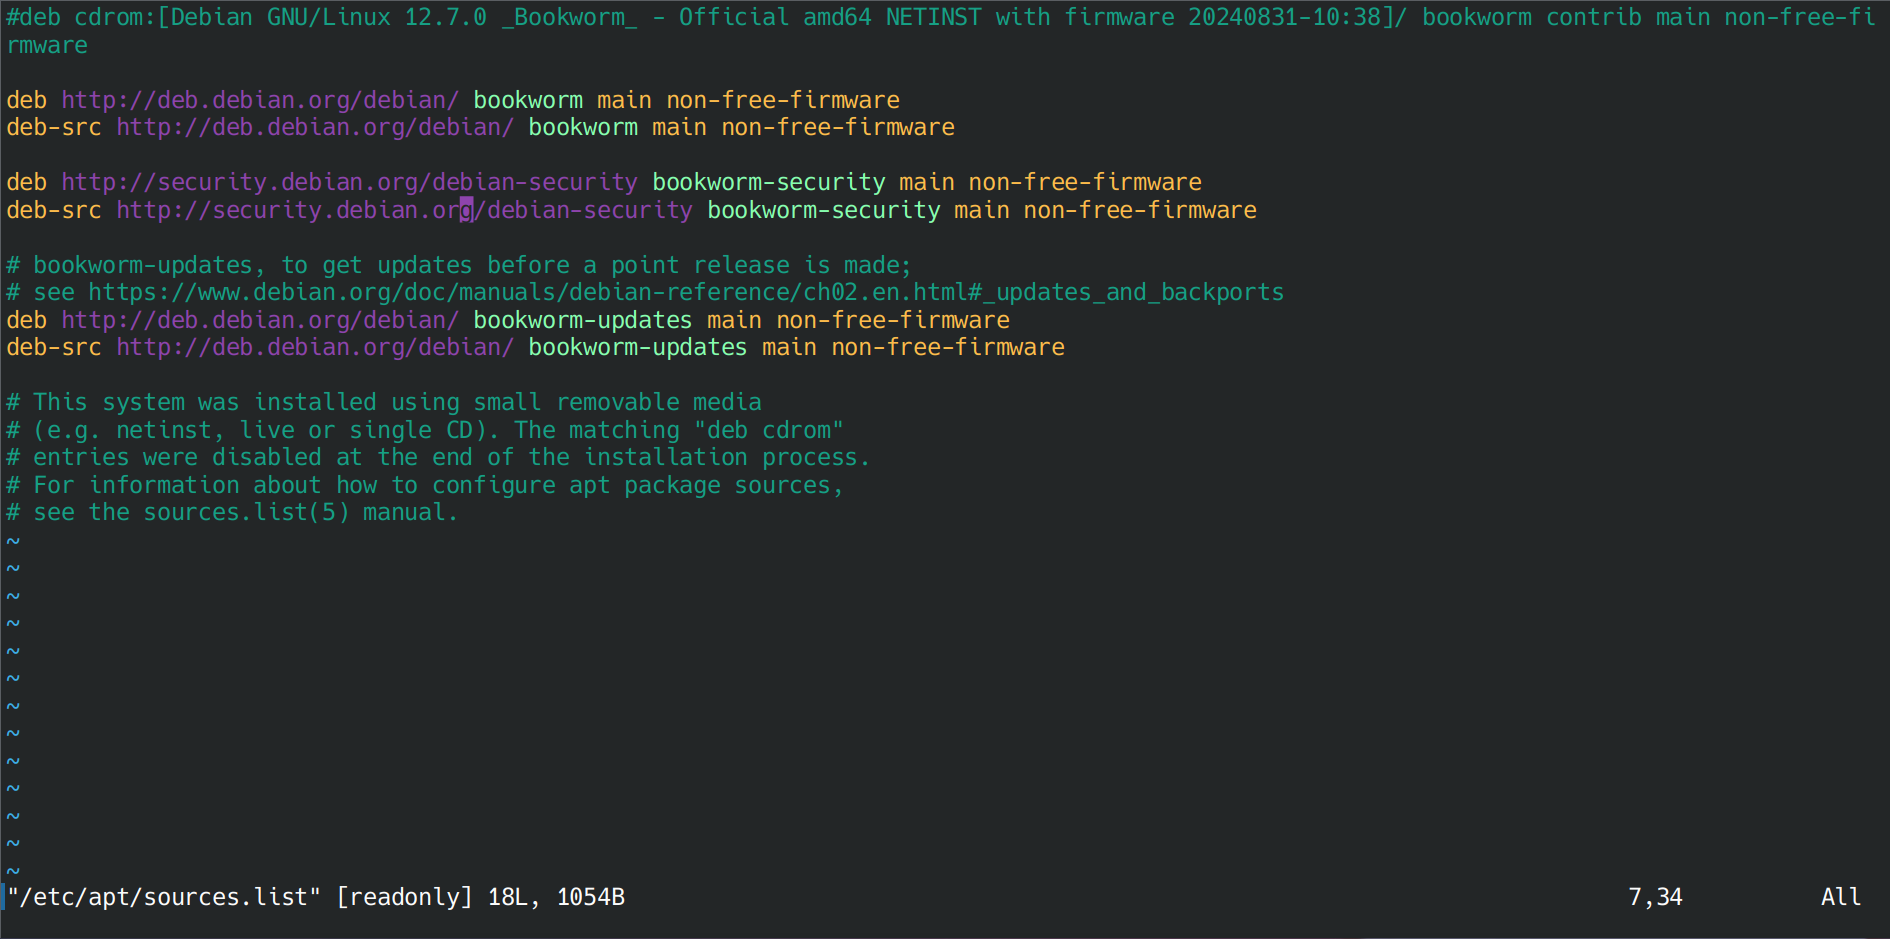
\includegraphics[scale=0.3]{figuras/source_list.png}
  \caption{Conteúdo do arquivo \textit{/etc/apt/sources.list}.}
  \label{fig:sources}
\end{figure}

\subsubsection{uname}
A Figura~\ref{fig:uname} mostra a saída do comando \textit{uname}, utilizado para exibir informações sobre o sistema operacional em execução~\cite{negus2012}. Este comando tem como saída detalhes sobre o sistema, como o nome do kernel, a versão do kernel, a arquitetura do processador e o nome do host. O parâmetro ''-a`` é usado para que a saída mostre todas as informações disponíveis.

\begin{figure}[H]
  \centering
  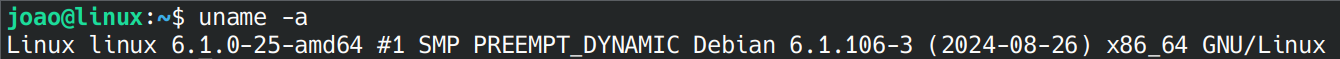
\includegraphics[scale=0.43]{figuras/uname.png}
  \caption{Saída do comando \textit{uname -a}.}
  \label{fig:uname}
\end{figure}

\subsubsection{Comandos Gerais}
Existem comandos fundamentais para a interação com o sistema operacional e a realização de diversas operações~\cite{guiafocaIniciante}. Abaixo, apresentamos uma lista de comandos comumente usados:

\begin{itemize}
    \item \texttt{clear}: Restaura o terminal a um estado inicial, ``limpando'' todas as saídas anteriores e comandos executados.

    \item \texttt{ls -l}: Exibe uma lista detalhada dos arquivos e diretórios no diretório especificado. Caso nenhum diretório seja indicado, a listagem será feita do diretório atual.

    \item \texttt{cd}: Altera o diretório de trabalho atual para o diretório especificado no parâmetro, permitindo a navegação pelo sistema de arquivos.

    \item \texttt{cat}: Concatena e exibe o conteúdo de um ou mais arquivos na saída padrão.

    \item \texttt{rm}: Remove permanentemente o arquivo especificado do sistema.

    \item \texttt{nano}: Editor de texto em linha de comando que permite a criação e modificação de arquivos de texto diretamente no terminal.

    \item \texttt{cp}: Copia um arquivo de origem para o destino especificado.

    \item \texttt{grep}: Busca e exibe as linhas de um arquivo que correspondem a um padrão especificado pelo usuário.

    \item \texttt{head}: Exibe as primeiras linhas de um arquivo, por padrão somente as 10 primeiras linhas são exibidas. 

    \item \texttt{tail}: Mostra as últimas linhas de um arquivo. Similar ao comando \texttt{head}, também exibe 10 linhas por padrão.

    \item \texttt{mv}: Move ou renomeia arquivos. 
\end{itemize}

A Figura~\ref{fig:comandos} e a Figura~\ref{fig:comandos2} ilustram o uso desses comandos.

\begin{figure}[H]
  \centering
  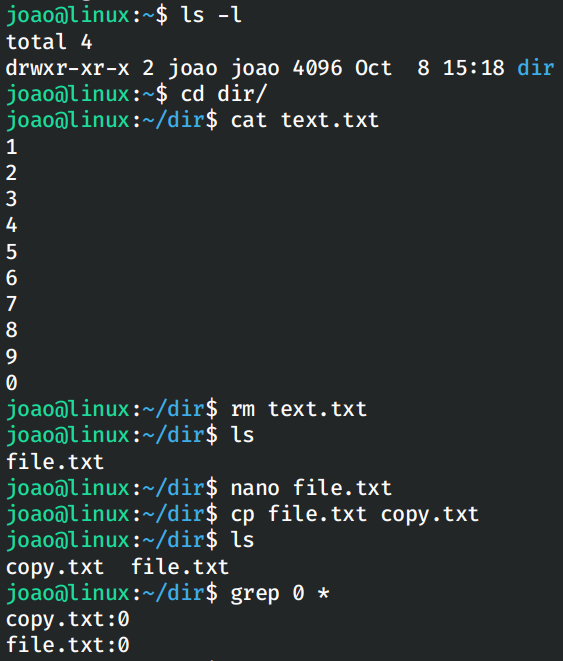
\includegraphics[scale=0.5]{figuras/commons.png}
  \caption{Exemplo de comandos gerais do Linux em um terminal.}
  \label{fig:comandos}
\end{figure}

\begin{figure}[H]
  \centering
  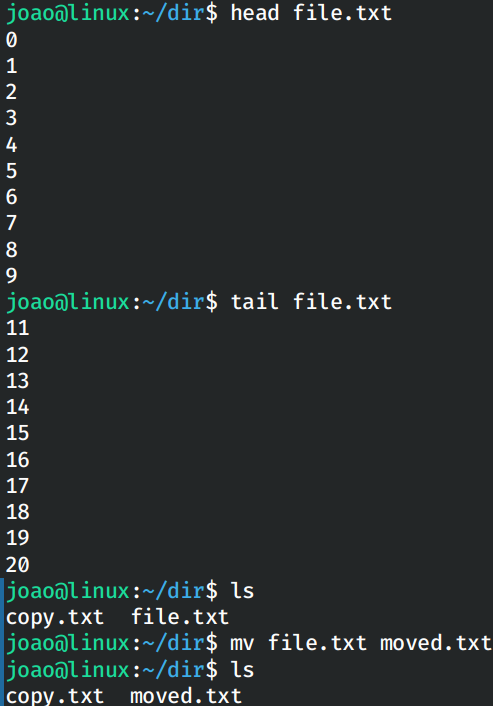
\includegraphics[scale=0.5]{figuras/commons2.png}
  \caption{Exemplo de comandos gerais do Linux em um terminal.}
  \label{fig:comandos2}
\end{figure}

\subsection{Compilação do Núcleo}
\label{subsec:compilacao}

Para o processo de compilação do núcleo Linux, é essencial instalar uma série de programas e bibliotecas necessárias. O comando utilizado para essa instalação é  o \textit{apt install build-essentials bc dwarves bison flex gnupg libncurses-dev libelf-dev libssl-dev wget}. Este comando instala um conjunto de pacotes no sistema, cada um com funções específicas que contribuem para a compilação e configuração do núcleo.

\begin{itemize}
    \item \texttt{build-essentials}: Um conjunto de pacotes essenciais para construção de pacotes no Debian.

    \item \texttt{bc}: Calculadora de linha de comando.

    \item \texttt{dwarves}: Conjunto de ferramentas depuração para arquivos no formato Executable and Linkable Format(ELF).

    \item \texttt{bison}: Gerador de analisador sintático de uso geral. 

    \item \texttt{flex}: Gerador de analisadores léxicos.
    
    \item \texttt{gnupg}: Ferramenta para encriptação de dados e geração de assinaturas digitais.

    \item \texttt{libncurses-dev}: Biblioteca de manipulação de caracteres em terminais.

    \item \texttt{libelf-dev}: Biblioteca para leitura e escrita de arquivos ELF.
    
    \item \texttt{libssl-dev}: Parte do projeto OpenSSL para implementação do protocolo Secure Socket Layer(SSL) e Transport Layer Security (TLS).

    \item \texttt{wget}: Utilitário para obter arquivos usando Hypertext Transfer Protocol (HTTP) ou File Transfer Protocol (FTP).
\end{itemize}

Durante a realização deste trabalho, a versão mais recente do núcleo Linux disponível era a 6.10.11. A obtenção dessa versão foi realizada por meio do comando \textit{wget https://cdn.kernel.org/pub/linux/kernel/v6.x/linux-6.10.11.tar.xz}. O código-fonte é fornecido em um arquivo comprimido, requerendo sua extração. Isso pode ser feito com o comando \textit{tar -xf linux-6.10.11.tar.xz -C /usr/src/linux-6.10.11/}. A Figura~\ref{fig:wget} ilustra este processo.

\begin{figure}[H]
  \centering
  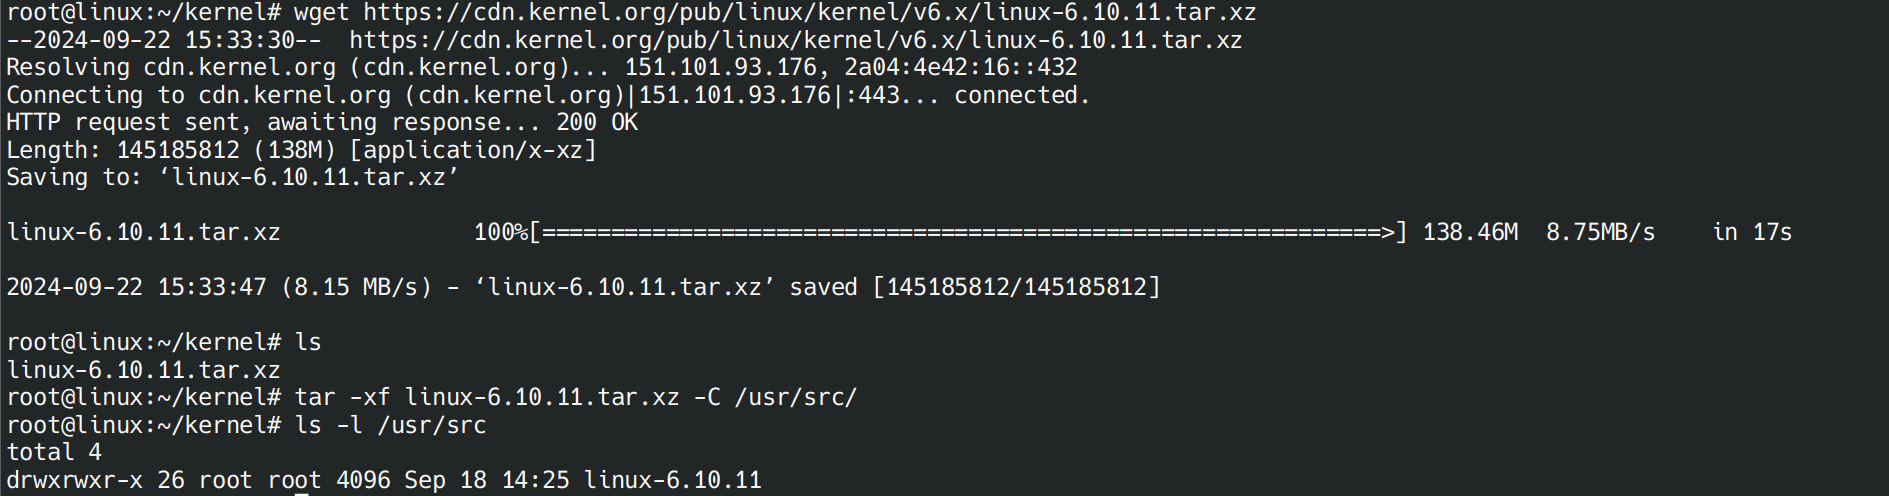
\includegraphics[scale=0.3]{figuras/wget.png}
  \caption{Obtenção do núcleo e extração do código-fonte.}
  \label{fig:wget}
\end{figure}

A compilação do núcleo Linux é baseada em um arquivo de configuração, que no diretório de compilação é denominado por \textit{.config}. No Debian, esse arquivo pode ser encontrado no diretório \textit{/boot}, onde estão armazenados diversos parâmetros que serão utilizados durante o processo de compilação. Antes de iniciar a compilação, é necessário obter este arquivo de configuração e copiá-lo para o diretório onde a compilação será realizada, que neste trabalho é o diretório \textit{/usr/src/linux-6.10.11/}. Para isso, foi utilizado o comando \textit{cp /boot/config-\$(uname -r) .config}.

Após essa configuração inicial, o comando \textit{make localmodconfig} é executado. Esse comando ajusta o arquivo de configuração de modo que apenas os módulos já carregados no sistema sejam considerados durante a compilação.

Para as configurações de módulo o comando \textit{make menuconfig} é usado, com ele uma interface é apresentada para o usuário de modo que o mesmo possa escolher algumas opções que serão ou não compiladas com o núcleo. Na Figura~\ref{fig:usb} temos o uso deste menu para a habilitação do módulo para Universal Serial Bus (USB) \textit{mass storage}, o que basicamente habilita o suporte para \textit{pen drive}, alguns tipos de dispositivos de disco rígido via USB e afins. Já a Figura~\ref{fig:ntfs} utiliza o menu para habilitar o NT File System (NTFS) um sistema de arquivos utilizado no Windows.

\begin{figure}[H]
  \centering
  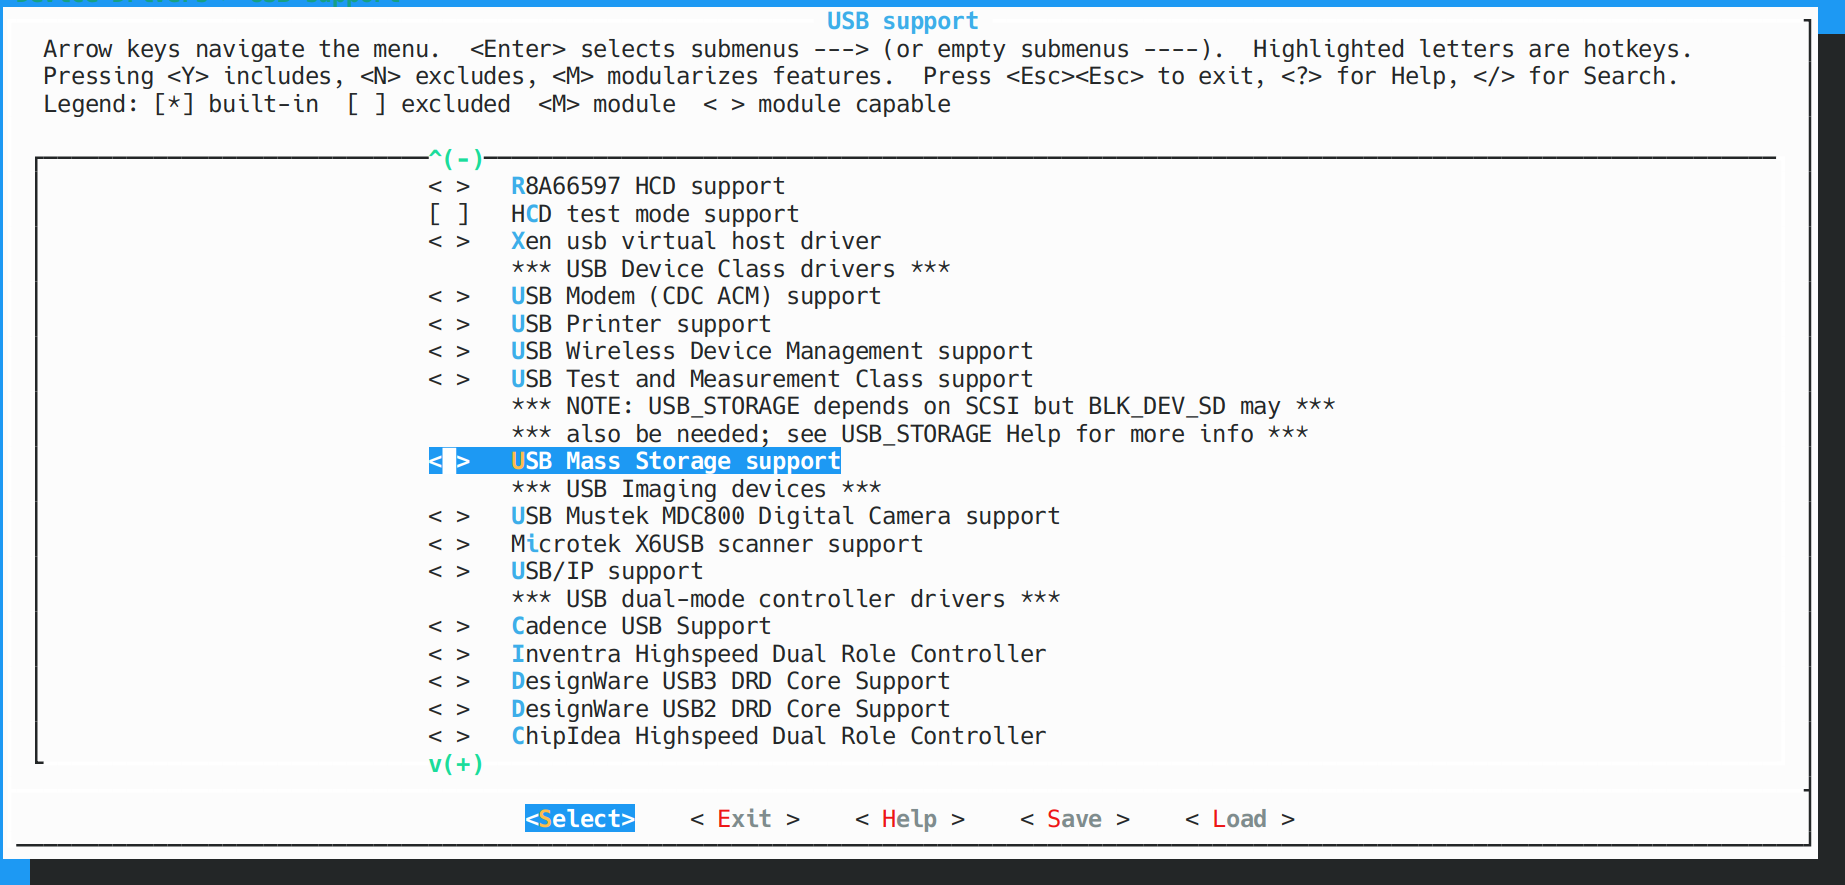
\includegraphics[scale=0.3]{figuras/usb.png}
  \caption{Habilitando módulo para USB \textit{mass storage}.}
  \label{fig:usb}
\end{figure}

\begin{figure}[H]
  \centering
  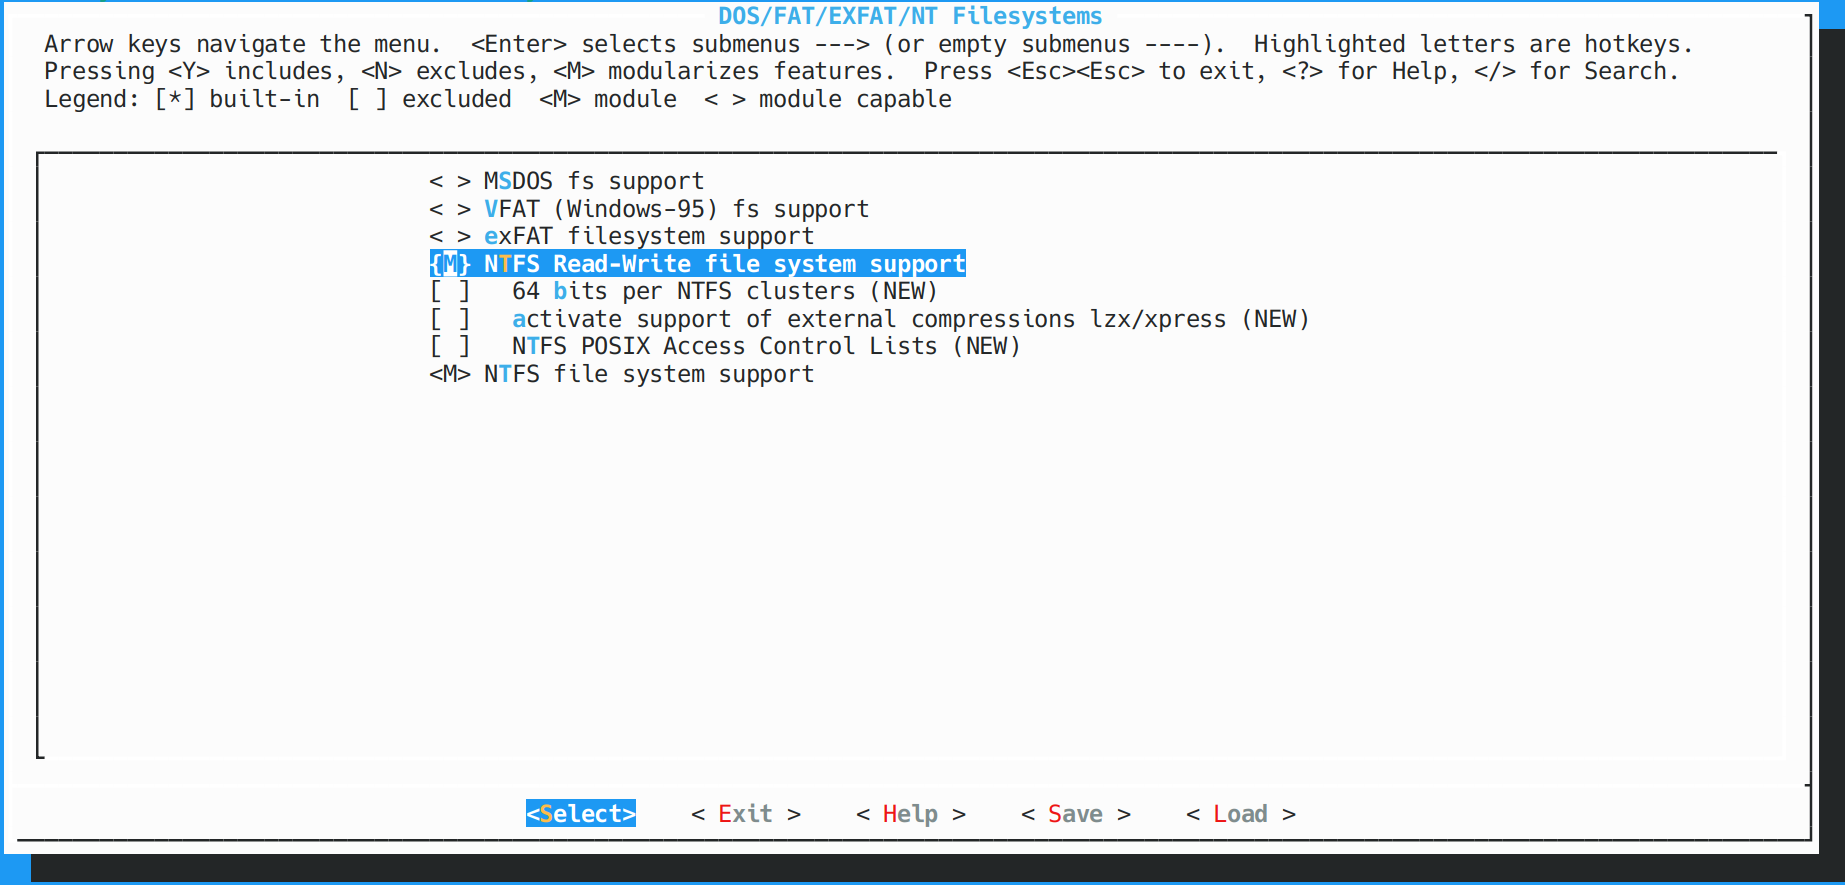
\includegraphics[scale=0.3]{figuras/ntfs.png}
  \caption{Habilitando módulo para sistema de arquivos NTFS.}
  \label{fig:ntfs}
\end{figure}

O uso deste menu não se limita apenas à habilitação de módulos importantes, mas também permite a desabilitação de módulos que não serão utilizados. A Figura~\ref{fig:macintosh} ilustra a configuração necessária para desabilitar \textit{drivers} de dispositivos específicos para computadores Macintosh.

\begin{figure}[H]
  \centering
  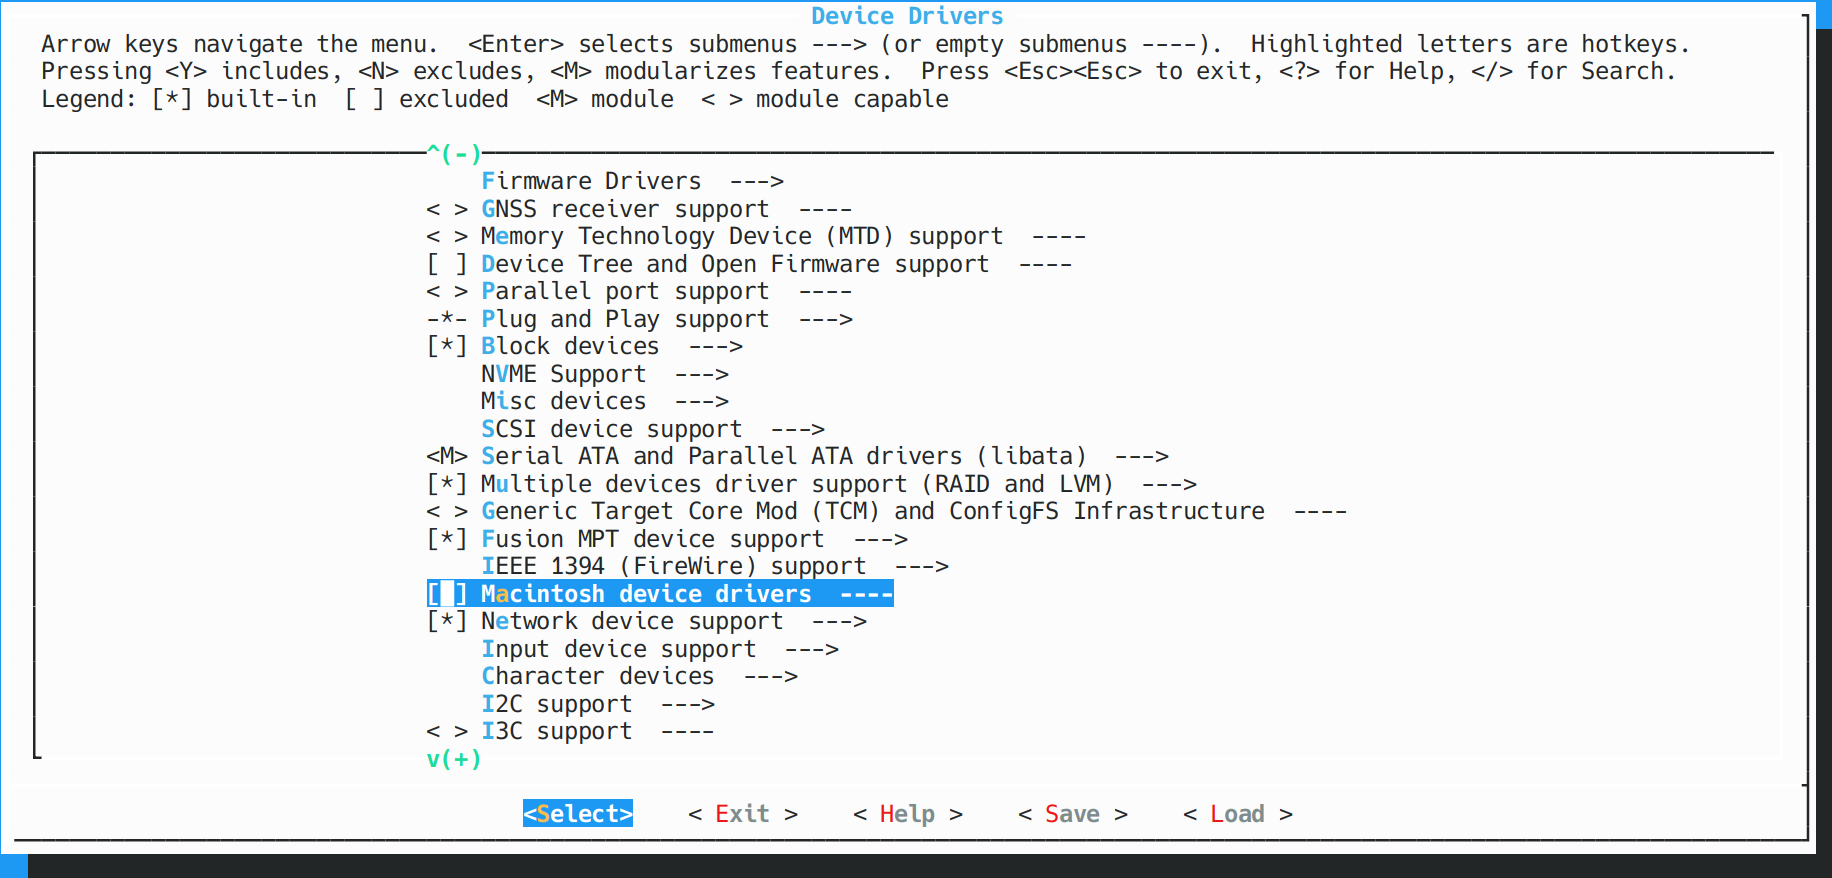
\includegraphics[scale=0.3]{figuras/macintosh.png}
  \caption{Desabilitando módulos de \textit{driver} para computadores Macintosh.}
  \label{fig:macintosh}
\end{figure}

Após as configurações no núcleo a compilação pode ser realizada. Na compilação do núcleo o comando \textit{make -j2 LOCALVERSION=-utfpr} foi utilizado, onde \textit{-j2} especifica a quantidade de núcleos utilizados durante a compilação e \textit{LOCALVERSION=-utfpr} é um parâmetro opcional que especifica um nome que será concatenado ao nome do núcleo.

Após as configurações no núcleo, o processo de compilação pode ser iniciado. Para isso, foi utilizado o comando \textit{make -j2 LOCALVERSION=-utfpr}. Nesse comando, ``-j2'' especifica o número de núcleos a serem utilizados durante a compilação, otimizando o tempo de execução. O parâmetro opcional \textit{LOCALVERSION=-utfpr} adiciona um sufixo ao nome do núcleo, facilitando a identificação da versão compilada.

Uma vez concluída a compilação, o comando \textit{make modules\_install} deve ser utilizado para instalar os módulos do núcleo compilado. Em seguida, o comando \textit{make install} instala o núcleo em si. Vale ressaltar que o novo núcleo só será utilizado após a reinicialização da máquina. A Figura~\ref{fig:uname_pos} mostra a saída do comando \textit{uname -a} após a reinicialização do comando.

\begin{figure}[H]
  \centering
  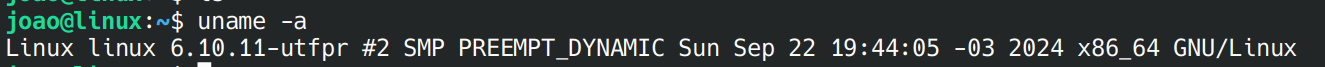
\includegraphics[scale=0.3]{figuras/uname_pos.png}
  \caption{Saída do comando \textit{uname -a} após a compilação do núcleo.}
  \label{fig:uname_pos}
\end{figure}

A Figura~\ref{fig:boot} mostra a saída do comando \textit{du -sh /lib/modules/6.10.11-utfpr/} que retorna o espaço em disco ocupado pelos módulos do núcleo, e também a saída do comando \textit{ls -lh /boot} que têm como saída os arquivos essenciais para o funcionamento do núcleo, nele encontramos duas versões do núcleo sobre o nome \textit{vmlinuz}, as configurações de compilação do mesmo sobre o nome \textit{config} o \textit{initrd} usado para iniciar o sistema operacional e por fim \textit{System.map} que armazena alguns símbolos do núcleo para facilitar a depuração~\cite{linuxKernel}.

\begin{figure}[H]
  \centering
  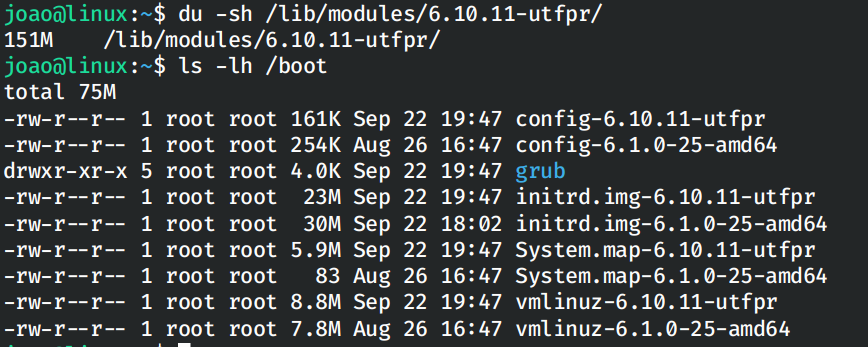
\includegraphics[scale=0.3]{figuras/boot.png}
  \caption{Obtenção do núcleo e extração do código-fonte.}
  \label{fig:boot}
\end{figure}

\section{Discussão dos Resultados}
\label{sec:discussao}

\section{Conclusões}
\label{sec:conclusoes}

% ----------------------------------------------------------
% ELEMENTOS PÓS-TEXTUAIS
% ----------------------------------------------------------
\postextual
% ----------------------------------------------------------
% Referências bibliográficas
% ----------------------------------------------------------
\renewcommand{\bibsection}{%
\section{\bibname}
\bibmark
%\ifnobibintoc\else
%\phantomsection
%\addcontentsline{toc}{section}{\bibname}
%\fi
\prebibhook}

\bibliography{abntex2-modelo-references}

\end{document}
